
\section{Gameplay Mechanics}

\subsection{Level Generation}

The game will use elements of procedural generation to create levels. To do this, first a grid of \textit{rooms} is created as shown in figure~\ref{4x}. A random position on the top of the grid is chosen to be the starting room. From here there is a probability of stepping left/right or down. If the stepping algorithm reaches a wall it will automatically step down. At the bottom of the grid the probability of stepping down is replaced with the probability of creating a level end.

\begin{figure}[ht]
\centering
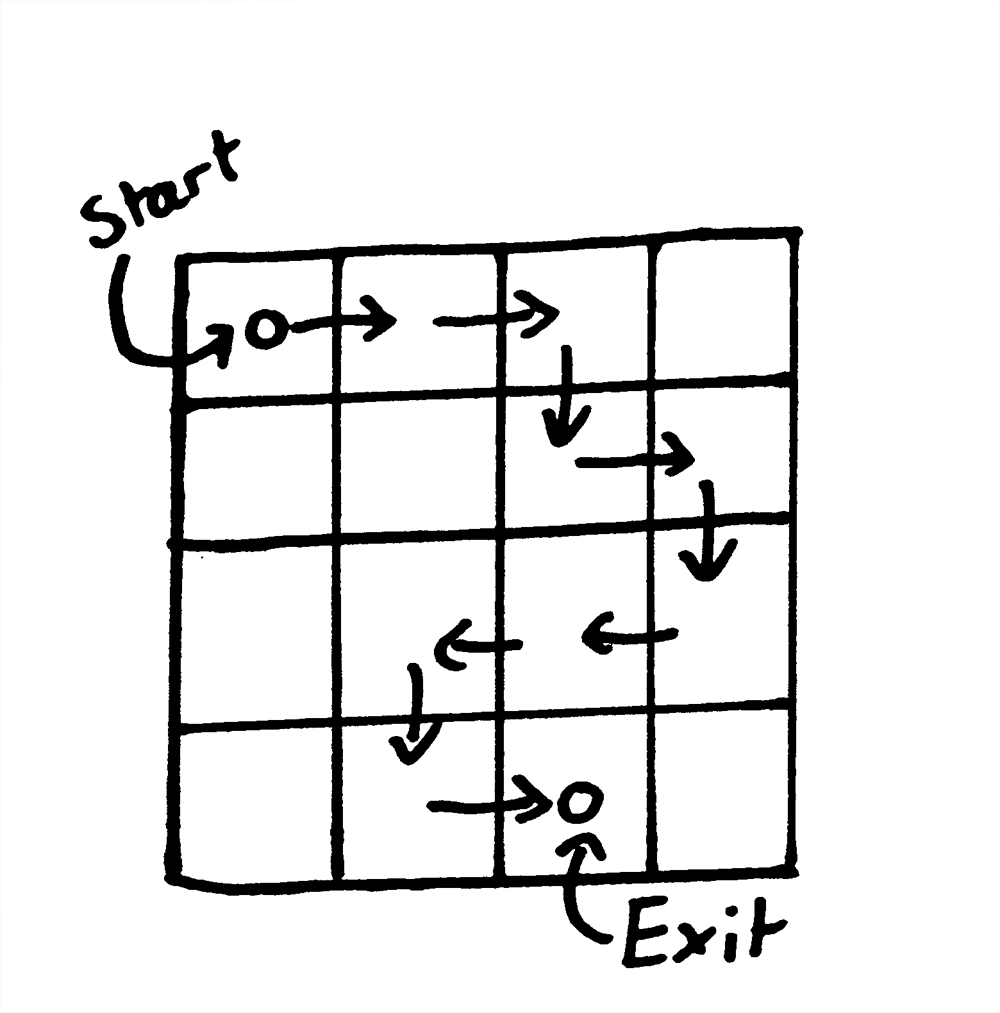
\includegraphics[scale=0.2, trim = 0cm 0cm 0cm 5cm]{images/4x4}
\label{fig:4x}
\caption{Solution path generation}
\end{figure}

After the room grid is created the individual rooms are populated with pre-existing room tiles. To get a basic version of the game running only the four room tiles show in figure~\ref{16x} would be needed with solid rooms for the rooms off the solution path.

\begin{figure}[ht]
\centering
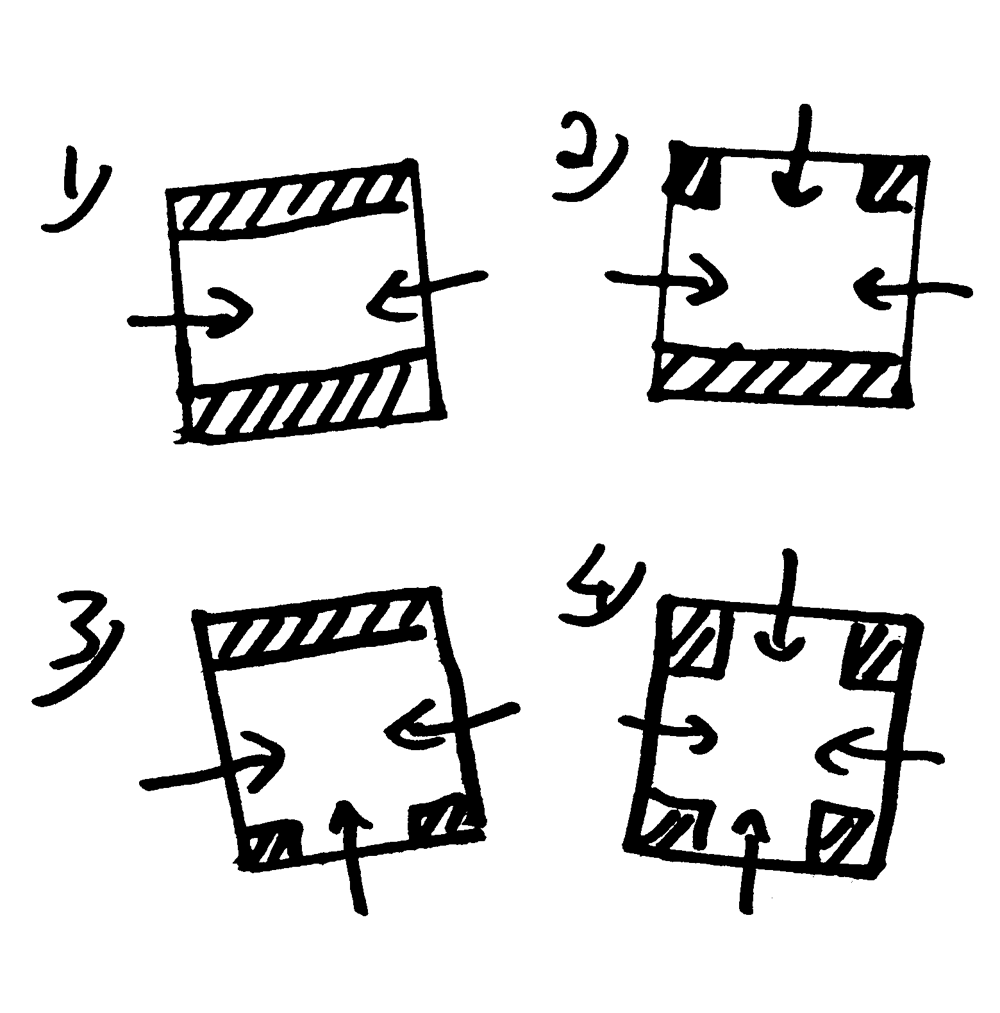
\includegraphics[scale=0.2, trim = 0cm 0cm 0cm 5cm]{images/16x16}
\label{fig:16x}
\caption{Basic tiles needed}
\end{figure}

Individual rooms will be tile based and will be stored in text files which the game will read in and then populate.
